\section{Materials and Methods}


% \begin{figure}[!htb]
%     \centering
%     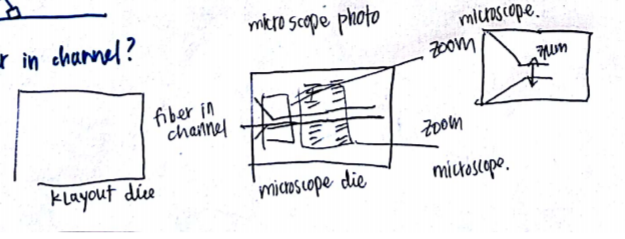
\includegraphics[width=1\columnwidth]{images/cartoon/die_klayout.png}
%     \vspace{0mm}
%     \caption{Layout and fabricated designs. (a) Microelectrode actuator design in layout. (b) The fabricated design. (c) Detail showing insertion funnel for loading carbon fibers. (d) Detail showing angled arm design with carbon fiber in the channel.}
%     \label{fig:die-klayout}
% \end{figure}


\begin{figure}[]
    \centering
    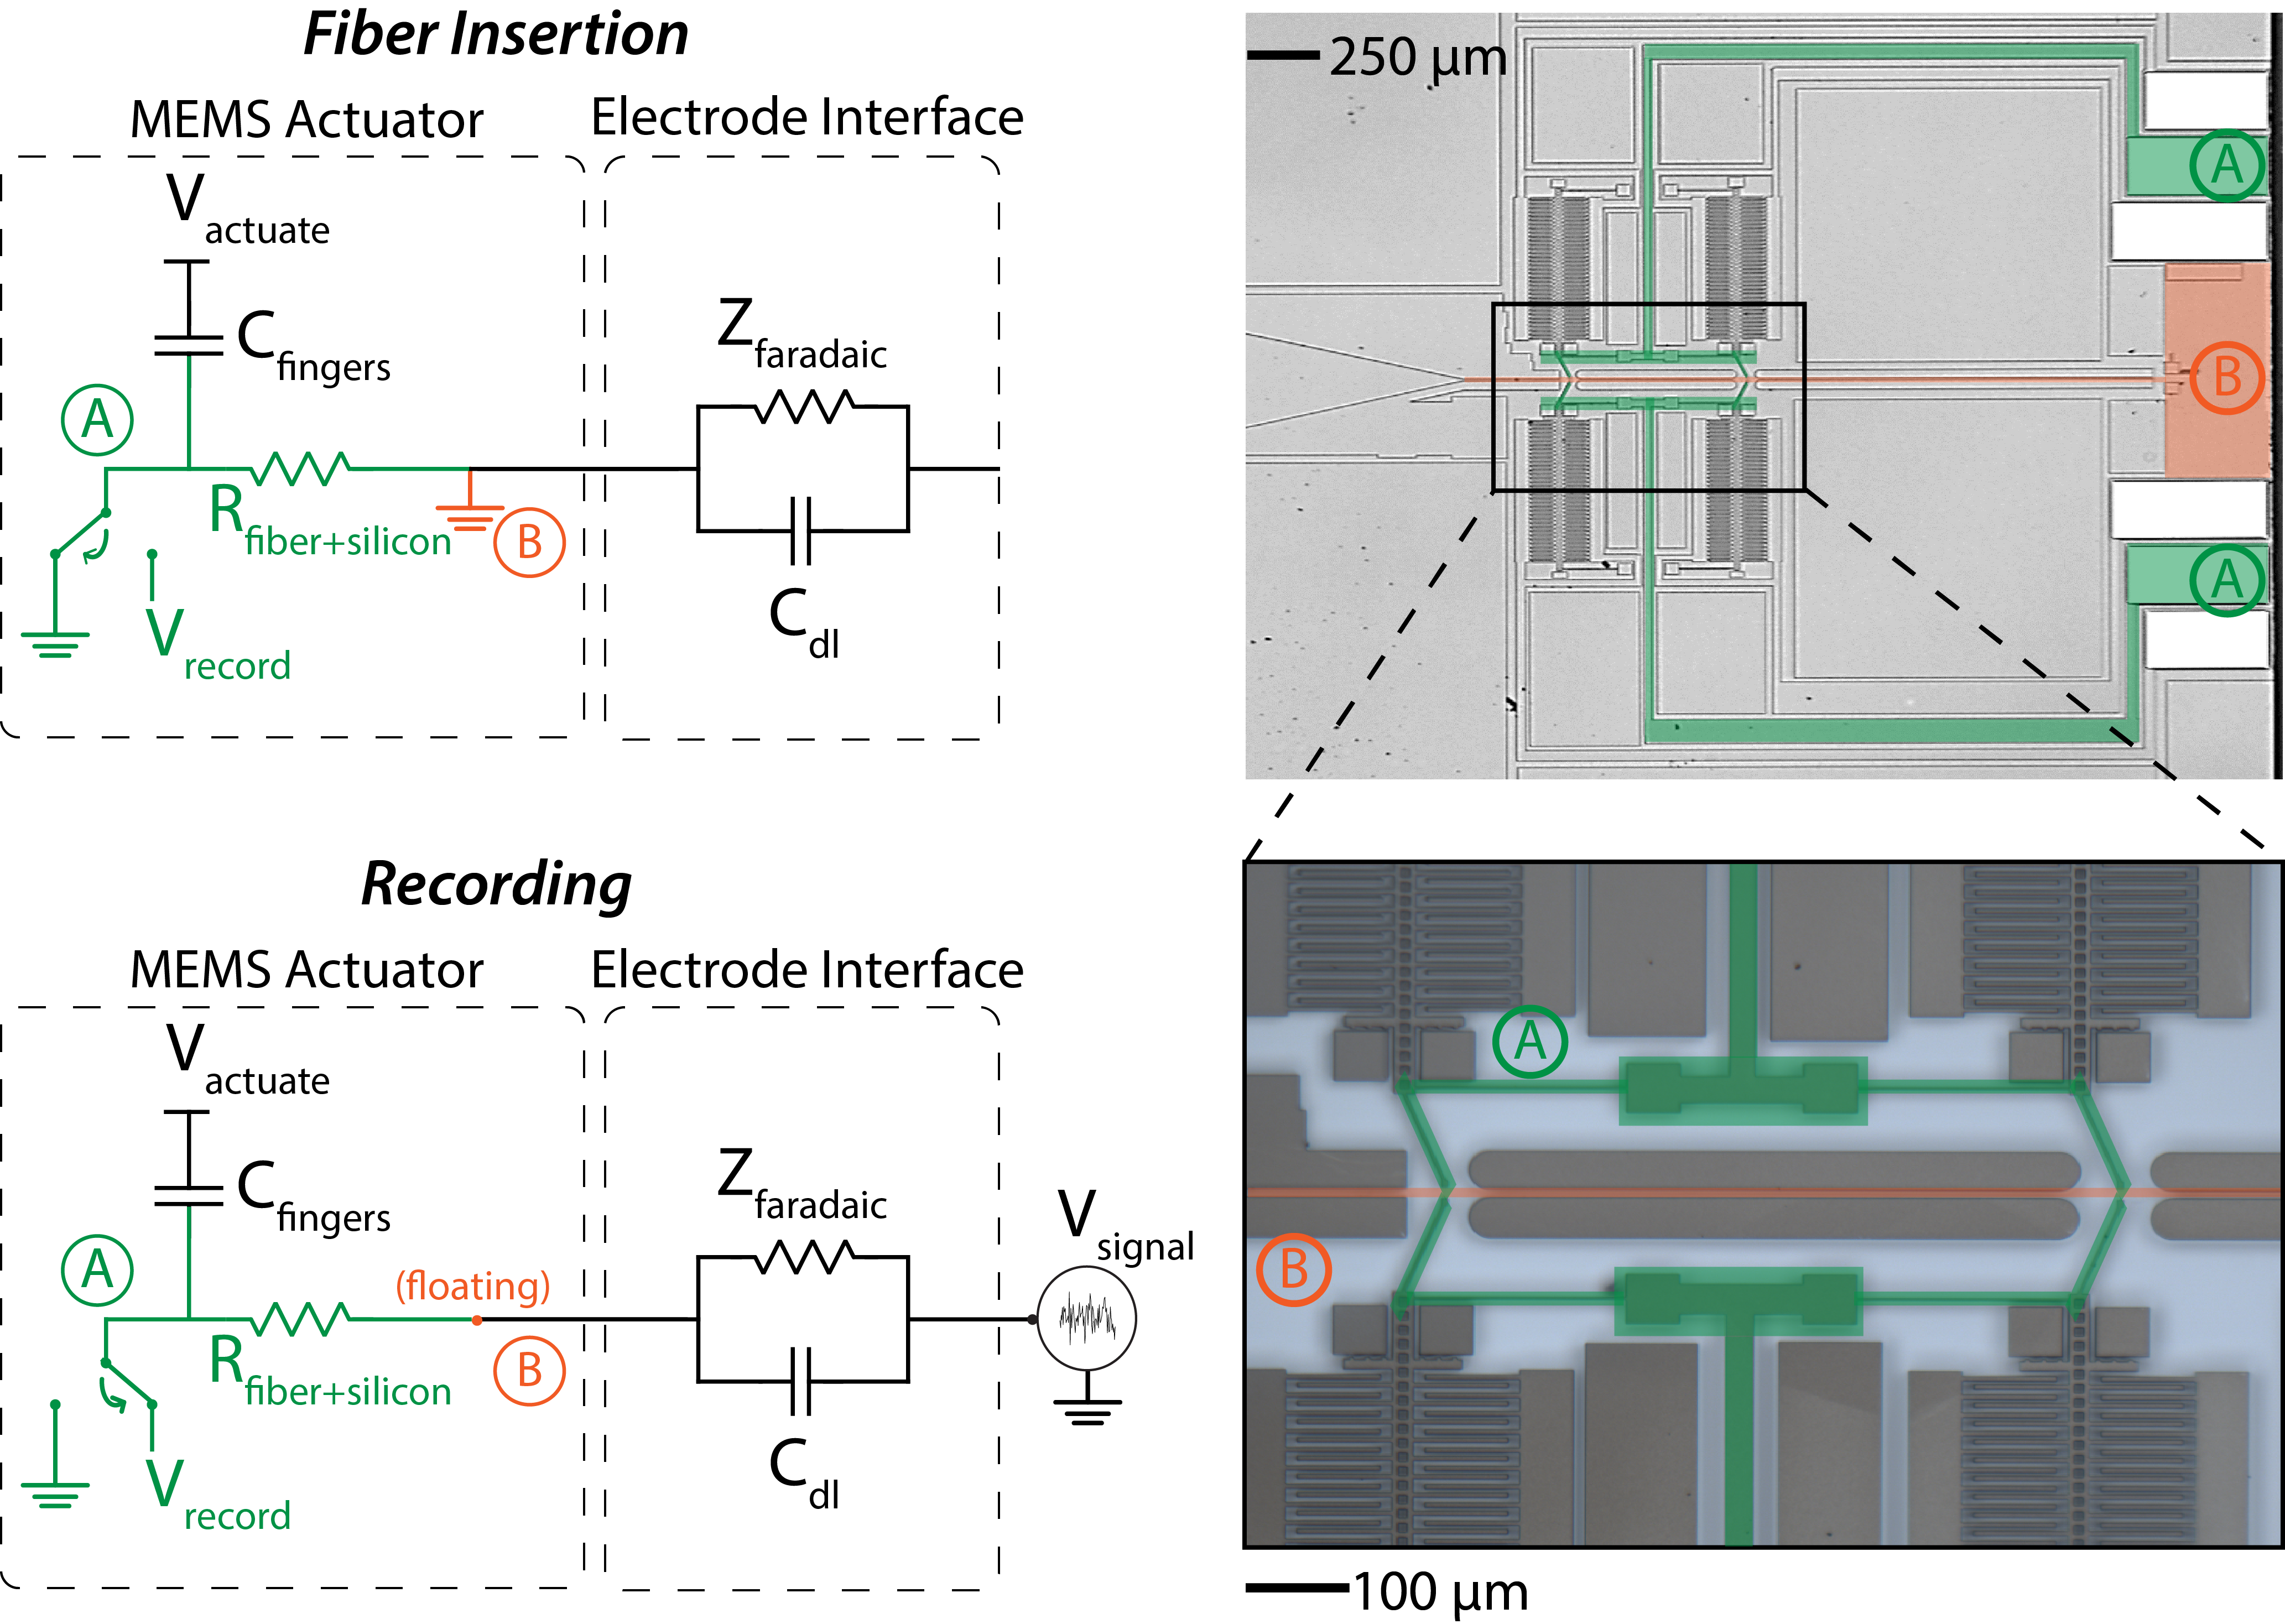
\includegraphics[width=\columnwidth]{images/cartoon-2stages-dd.png}
    \caption{Left: Equivalent circuit models of the device. During fiber insertion (top), the electrostatic actuator pushes the fiber forwards in channel. During recording (bottom), neural signals are captured by closing all four angled arms until they contact the carbon fiber. Electrically connected segments have been labelled and highlighted. ``A'', green, represents the silicon traces and angled arms which contact the carbon fiber; ``B'', orange, represents the carbon fiber channel and substrate. Right: Image of the device, with inset shown at bottom.}
    \label{fig:cartoon-2states}
\end{figure}

\subsection{Theory of Operation}
\todo{update this section}

    %\todo{Make sure figures are all spaced appropriately}
    \subsubsection{Fiber Insertion}

    In this work, we designed a MEMS actuator containing an electrostatic motor with angled arms, as in~\cite{Penskiy2013, Schindler2017}. The electrostatic motors presented here are capable of producing millinewton forces over many millimeters of travel~\cite{Yeh2002, Penskiy2013, Contreras2017, Schindler2017}, sufficient for the penetration forces (calculated to be on the order of hundreds of micronewtons for this electrode style) and depths necessary for most applications~\cite{Massey2018,Patel2016,Kozai2012}. In prior work, these actuators have been used to advance \SI{7.2}{\micro\meter} carbon fibers in air, but have not been characterized for their mechanical insertion and electrical characteristics in the context of neural recording \cite{Schindler2017}.
    
    Each actuation cycle of the electrostatic motor pushes the fiber a small distance. Motion is achieved by applying voltage to an interdigitated set of capacitive fingers. Initially, one set of fingers is grounded, while the other set is held at V$_{actuate}$. This electrostatic force causes the interdigitated capacitive fingers to pull in towards one another, in turn pushing out a set of flexible angled arms which grip the carbon fiber. To disengage the flexible arms from the carbon fiber, both sets of capacitive fingers are grounded and a spring pulls the capacitive fingers apart. 
    
    By using two such actuators to perform a cyclic motion in which the angled arms come into contact with the carbon fiber, move it forwards one step, disengage, and return to their initial position, the motor accumulates small steps which eventually advance the microelectrode over a large distance. For more details on actuation, see~\cite{Penskiy2013}.

    % then translated to the carbon fiber via two sets of flexible angled arms, which correspondingly grip and release the fiber in anti-phase to accumulate small forwards motions. As seen in \todo{some figure in this text which diagrams gap closers actuating vertically, shuttle pushed horizontally}, the movement of GCAs is perpendicular to that of the carbon fiber; however, the angled arm applies force in both the transverse and longitudinal directions. Transverse forces produced by opposite sets of actuators are cancelled out, producing a net longitudinal force. Silicon springs provide a restoring force when high-voltage is removed~\cite{Penskiy2013}. 

    % Discussion of connections
    
    Fig.~\ref{fig:cartoon-2states} shows equivalent circuit diagrams (left) and corresponding images of the device (right) with electrically connected segments labelled and highlighted.
    
    During insertion of a fiber (Fig.~\ref{fig:cartoon-2states}, top left), the silicon angled arms and one set of capacitive fingers in each actuator are tied to ground (highlighted in green, ``A''). The other set of capacitive fingers alternates between V$_{actuate}$ and ground, dictating whether the angled arms are in contact with or disengaged from the carbon fiber. The substrate (highlighted in orange, ``B'') is also grounded to prevent released silicon structures from electrostatically pulling in to the substrate.
    
    In Fig.~\ref{fig:cartoon-2states} (top right), the green highlighted regions indicate the signal path from the wirebond pads, through the silicon traces, to the angled arms which contact the carbon fiber. The orange highlighted regions indicate the substrate connection and location of a carbon fiber within the channel. Fig.~\ref{fig:cartoon-2states} (bottom right) shows an inset of the silicon traces and angled arms (green) which come in contact with the fiber, nominally held in place in the fiber channel (orange).

    When no voltage is applied to the actuator motor, the carbon fiber is not in contact with any silicon structure other than the substrate.
    
    \subsubsection{Recording}
    When recording signals from the electrode (Fig.~\ref{fig:cartoon-2states}, bottom left), all four angled arms make contact with the carbon fiber when a high voltage, V$_{actuate}$, is maintained across the capacitive fingers. These silicon arms, along with the corresponding silicon routing, form a signal path with which to record the neural signal. The path of impedance for this signal, from the tip of the carbon fiber in contact with the electrolyte to the external sensor circuity wire-bonded to the die, includes: parallel double-layer capacitance C$_{dl}$ and faradaic impedance Z$_{faradaic}$ at the electrode-electrolyte interface; carbon fiber impedance R$_{fiber+silicon}$; contact resistance between the carbon fiber and silicon angled arms; silicon traces; and wire bonds (all included in R$_{fiber+silicon}$). 
    
    The electrophysiological potential is recorded from the signal pad (green, ``A'') versus a reference electrode. The substrate and carbon fiber channel (orange, ``B'') are left floating to prevent grounding of the recorded signal. Although the voltage difference between the sets of capacitive fingers becomes V$_{actuate}-$V$_{signal}$ due to the micro-to-millivolt amplitude of neural recordings, this voltage is still sufficient to allow the angled arms to grip the fiber.

\subsection{Device Fabrication and Assembly}
    The MEMS actuator was fabricated with a two-mask silicon-on-insulator (SOI) process. Commercial SOI wafers consisting of a silicon substrate (\SI{550}{\micro\meter}), buried oxide layer (\SI{2}{\micro\meter}), and a device silicon layer (\SI{40}{\micro\meter}, \SI{3250}{\ohm}/$\square$), were used for all devices. First, aluminium was evaporated onto the wirebond sites to improve bond adhesion. Device silicon was lithographically patterned and etched using a deep reactive ion etch (DRIE). A subsequently patterned through-etch of the silicon substrate layer, also via DRIE, served to singulate the devices. Finally, a timed vapor HF etch was used to release the structures. The fabricated device is shown in Fig.~\ref{fig:die-photo} and Fig.~\ref{fig:cartoon-2states} (right).

    Electrical connections were made by wirebonding signal wires from the chip to an off-chip set of interconnects. A substrate grounding wire and the chip were held in place with silver epoxy. Placement of the fiber within the channel was achieved by adhering a fiber to a silicone-coated tungsten micromanipulator probe tip. The probe tip and carbon fiber assembly was aligned to the left of the device layer funnel, lowered to the correct height above the chip, and inserted into the channel. %Care was taken to prevent silver epoxy from shorting along the gold-coated interconnects.
    %The epoxy was cured at \SI{150}{\celsius} for \SI{10}{\minute}.
    %with \SIrange{8}{10}{\milli\meter} of carbon fiber extended beyond the edge of the probe tip. 
    %The entire chip assembly, including glass slide surface, grounding wire, MEMS chip, gold interconnects and wirebonds, is mounted on a vacuum chuck to provide stability during fiber insertion. 
    
    %Finally, the probe tip was separated from the fiber by lifting it out of plane.
    The chip is \SI{4.5}{\milli\meter} by \SI{3.5}{\milli\meter}, and has a mass of \SI{22}{\milli\gram}. The actuator/motor area is approximately \SI{1.5}{\square\milli\meter}.
    
\begin{figure}[t]
\centering
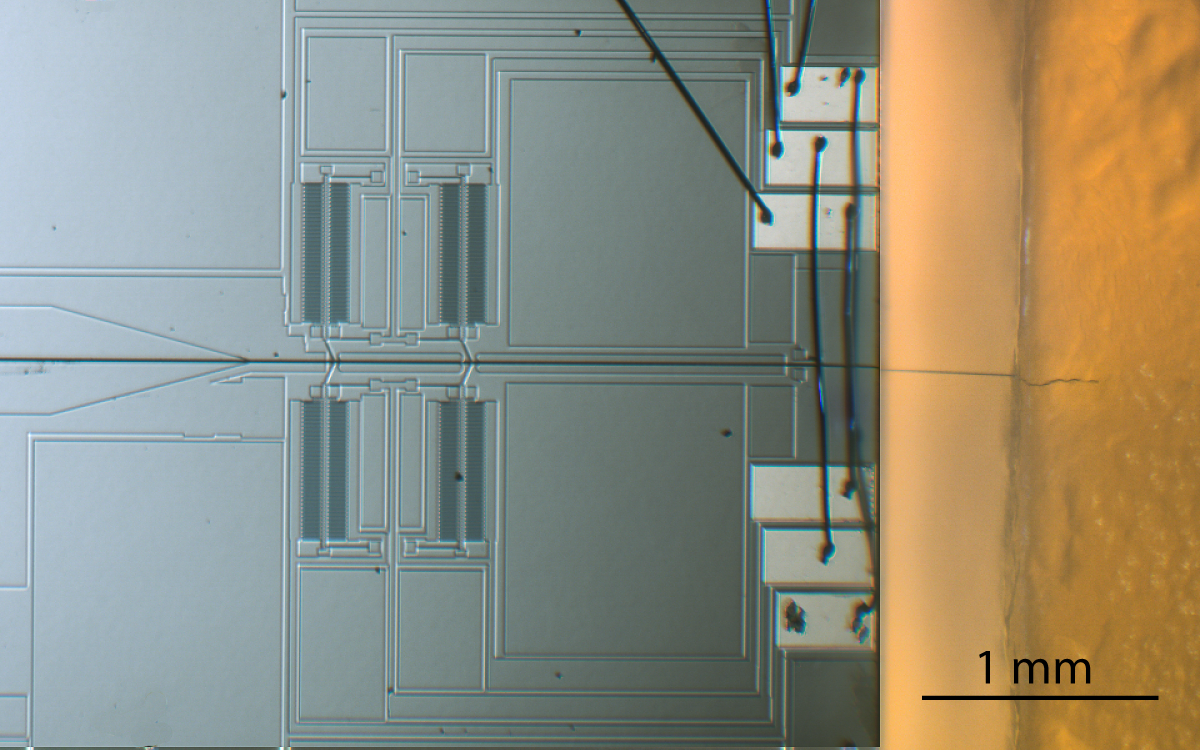
\includegraphics[width=\columnwidth]{images/CompositeFin.png}
\caption{The MEMS actuator and a \SI{7.2}{\micro\meter} diameter carbon fiber inserted approximately \SI{400}{\micro\meter} into the agar brain phantom.}
\label{fig:agar-push-composite}
\end{figure}

    
    